\documentclass[a4paper,10pt]{article}
\usepackage{geometry}
\geometry{margin=1cm}
\setlength{\parindent}{0pt} % kein indent bei absätzen
\setlength{\parskip}{\baselineskip} % abstand zwischen absätzen
\linespread{0.95} % controls the tightness overall


\usepackage{tikz}
\usetikzlibrary{shapes.geometric, arrows, positioning}

\tikzstyle{startstop} = [
	rectangle, 
	rounded corners, 
	minimum width=3.3cm,
	minimum height=1cm, 
	align=center, 
	text centered, 
	draw=black, 
	fill=gray!20]

\tikzstyle{process} = [
	rectangle, 
	minimum width=3.3cm, 
	minimum height=1cm,
	text centered, 
	align=center, 
	draw=black, 
	fill=blue!10]

\tikzstyle{decision} = [
	diamond, 
	aspect=2, 
	draw=black, 
	fill=yellow!20,
	align=center, 
	text centered, 
	inner sep=1pt]

\tikzstyle{arrow} = [->, thick]

\begin{document}

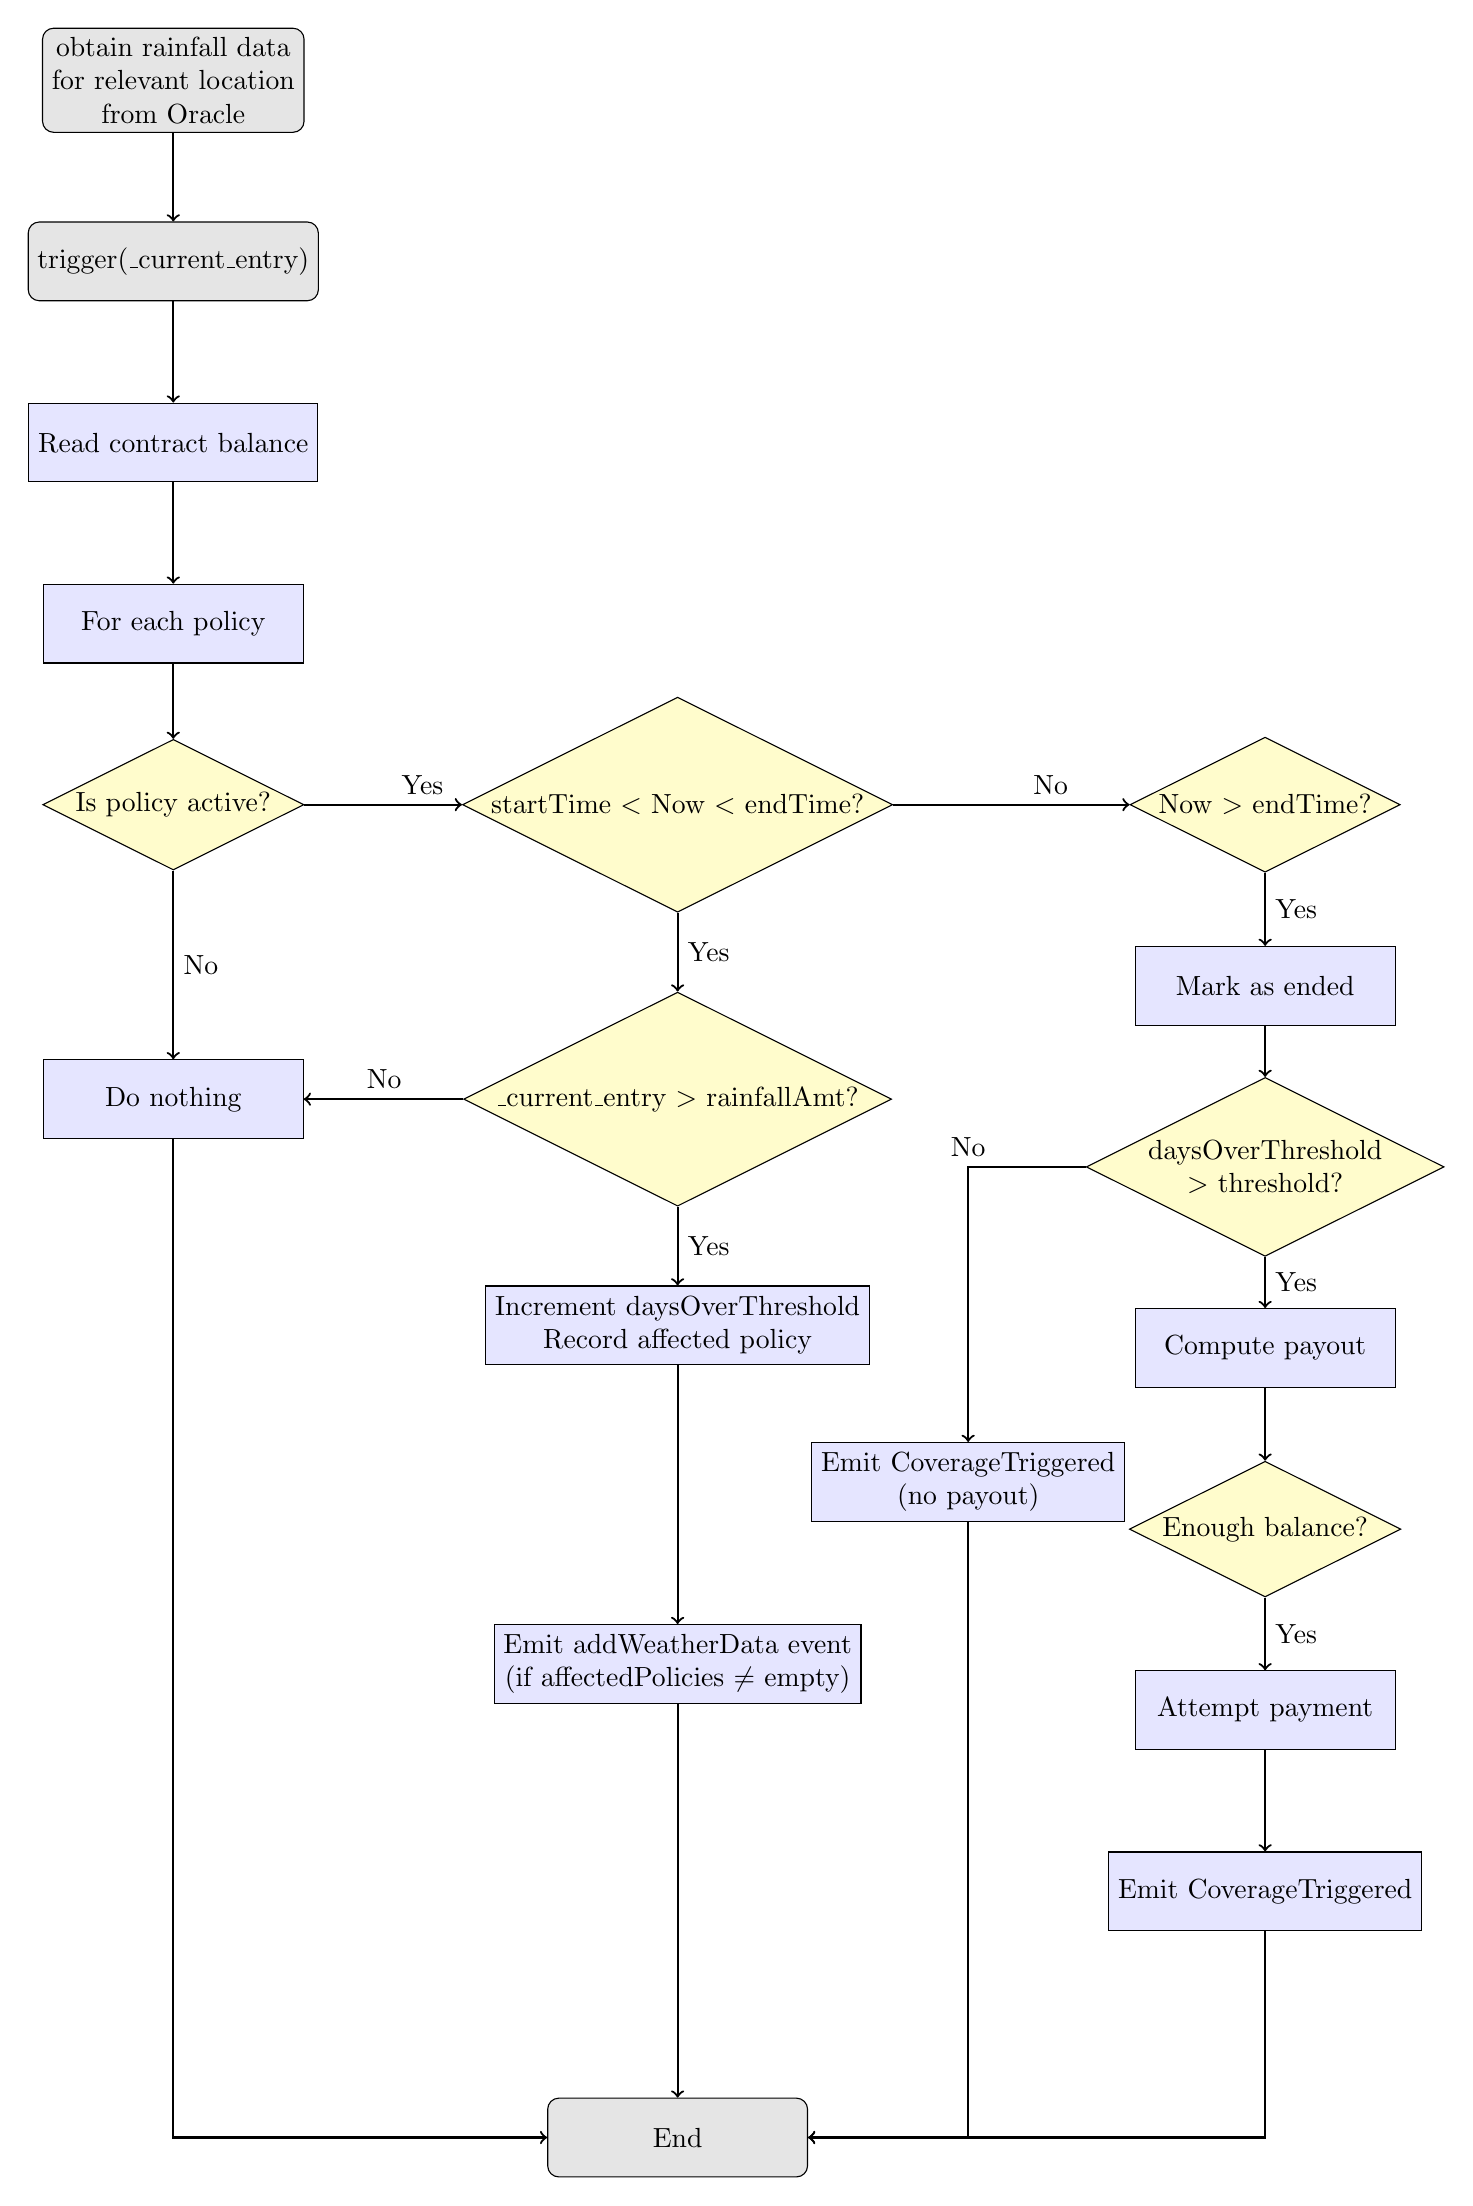
\begin{tikzpicture}[node distance=2.3cm]

% --- Nodes ---
\node (init) [startstop]  {obtain rainfall data \\ for relevant location \\ from Oracle};
\node (start) [startstop, below of=init] {trigger(\_current\_entry)};
\node (balance) [process, below of=start] {Read contract balance};
\node (loop) [process, below of=balance] {For each policy};

\node (before) [decision, below of=loop] {Is policy active?};
\node (nostart) [process, below=2.39635cm of before] {Do nothing};

\node (active) [decision, right=2cm of before] {startTime \textless{} Now \textless{} endTime?};
\node (rain) [decision, below= 1cm of active] {\_current\_entry \textgreater{}  rainfallAmt?};
\node (increment) [process, below=1cm of rain] {Increment daysOverThreshold \\ Record affected policy};

\node (expired) [decision, right=3cm of active] {Now \textgreater{} endTime?};
\node (endmark) [process, below of=expired] {Mark as ended};

\node (qualify) [decision, below of=endmark] {daysOverThreshold \\ \textgreater{}  threshold?};
\node (payoutcalc) [process, below of=qualify] {Compute payout};
\node (funds) [decision, below of=payoutcalc] {Enough balance?};
\node (send) [process, below of=funds] {Attempt payment};
\node (emitcov1) [process, below of=send] {Emit CoverageTriggered};

\node (emitcov2) [process, left =-0.5cm of qualify, yshift=-4cm] {Emit CoverageTriggered \\ (no payout)};

\node (emitweather) [process, below of=increment, yshift=-2cm] {Emit addWeatherData event \\ (if affectedPolicies $\neq$ empty)};

\node (end) [startstop, below=5cm of emitweather] {End};

% --- Arrows ---
\draw [arrow] (init) -- (start);

\draw [arrow] (start) -- (balance);
\draw [arrow] (balance) -- (loop);
\draw [arrow] (loop) -- (before);

\draw [arrow] (before) -- node[right]{No} (nostart);
\draw [arrow] (nostart.south) |- (end);

\draw [arrow] (before.east) -- ++(1,0) -- (active.west) node[midway,above]{Yes};

\draw [arrow] (active) -- node[right]{Yes} (rain);
\draw [arrow] (rain) -- node[right]{Yes} (increment);

\draw [arrow] (increment.south) -- ++(0,-1) -- (emitweather);

\draw [arrow] (rain.west) -- ++(-1,0) |- (nostart) node[midway,above]{No};

\draw [arrow] (active.east) -- ++(1,0) -- (expired.west) node[midway,above]{No};

\draw [arrow] (expired) -- node[right]{Yes} (endmark);
\draw [arrow] (endmark) -- (qualify);

\draw [arrow] (qualify) -- node[right]{Yes} (payoutcalc);
\draw [arrow] (qualify.west) -- ++(0,0) -| (emitcov2.north) node[midway,above]{No};

%\draw [arrow] (qualify.west) -- ++(-1,0) |- node[right]{No} (emitcov2);


\draw [arrow] (payoutcalc) -- (funds);

\draw [arrow] (funds) -- node[right]{Yes} (send);
\draw [arrow] (send) -- (emitcov1);
\draw[arrow] (emitcov1.south)-- ++(0,0) |- (end.east);
\draw[arrow] (emitcov2.south)-- ++(0,0) |- (end.east);

%\draw [arrow] (emitcov1.south) |- (emitweather);

%\draw [arrow] (funds.west) -- ++(-1,0) |- (emitcov2) node[midway,above]{No};
%\draw [arrow] (emitcov2) |- (emitweather);

%\draw [arrow] (expired.south) -- ++(0,-1) |- (emitcov2) node[pos=0.2,right]{No};

\draw [arrow] (emitweather) -- (end);

\end{tikzpicture}

\end{document}
